\documentclass[12pt, twoside]{article}
\usepackage[letterpaper, margin=1in, headsep=0.5in]{geometry}
\usepackage[english]{babel}
\usepackage[utf8]{inputenc}
\usepackage{amsmath}
\usepackage{amsfonts}
\usepackage{amssymb}
\usepackage{tikz}
\usetikzlibrary{quotes, angles}
\usepackage{graphicx}
%\usepackage{pgfplots}
%\pgfplotsset{width=10cm,compat=1.9}
%\usepgfplotslibrary{statistics}
%\usepackage{pgfplotstable}
%\usepackage{tkz-fct}
%\usepackage{venndiagram}
\usepackage{enumitem}
\usepackage{multicol}


\usepackage{fancyhdr}
\pagestyle{fancy}
\fancyhf{}
\fancyhead[LE]{\thepage}
\fancyhead[RO]{\thepage \\Name: \hspace{4cm} \,\\}
\fancyhead[LO]{BECA / Dr. Huson / Geometry 10th Grade\\* Unit 10: Trigonometry \& analytic geometry \\ 11 March 2020}

\renewcommand{\headrulewidth}{0pt}

\begin{document}
\subsubsection*{10.3 Do Now: Linear equations, review}
  \begin{enumerate}


  \item Write down the slope perpendicular to the given slope. \vspace{0.5cm}
  \begin{enumerate}
    \begin{multicols}{2}
    \item   $m= -\frac{3}{5} \hspace{1cm} m_{\perp} = $ \vspace{1cm}
    \item   $m= -2 \hspace{1cm} m_{\perp} = $
    \item   $m= 0.75 \hspace{1cm} m_{\perp} = $ \vspace{1cm}
    \item   $m= \frac{1}{2} \hspace{1cm} m_{\perp} = $
    \end{multicols}
  \end{enumerate}

  \item Write down the center and radius of each circle.
  \begin{enumerate}
    \begin{multicols}{2}
    \item   $(x+4)^2+(y-3)^2=81$ \vspace{2cm}
    \item   $x^2+(y+1)^2=20$
    \item   $x^2+8x+y^2-6y=-16$ \vspace{2cm}
    \item   $x^2-10x+y^2-16y=-40$
    \end{multicols}
  \end{enumerate}  \vspace{2cm}

  In the following problems, use the point-slope formula: $y-y_1=m (x-x_1)$
  \item What is the equation of a line through $(-1,-4)$ parallel to the line $y=\frac{3}{2}x+1$?  \vspace{2cm}
  \item What is the equation of a line through $(3,-5)$ perpendicular to the line $x-2y=6$?  \vspace{3cm}
  
  \item \emph{Spicy} What is an equation of the perpendicular bisector of $\overline{AB}$ with $A(-2,5)$ and $B(4,-1)$? \vspace{2cm}

\newpage

\item Describe a rigid motion that maps $\triangle TIC$ onto $\triangle TOK$. 
  \begin{flushright}
      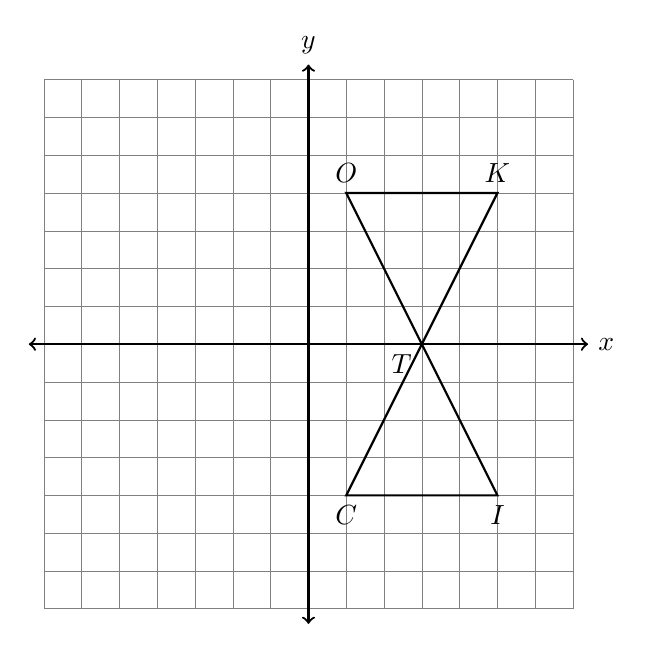
\begin{tikzpicture}[scale=.48]
      \draw [help lines] (-7,-7) grid (7,7);
      \draw [thick, <->] (-7.4,0) -- (7.4,0) node [right] {$x$};
      \draw [thick, <->] (0,-7.4)--(0,7.4) node [above] {$y$};  
      \draw [thick]
        (1,4) node[above] {$O$}--
        (5,4) node[above] {$K$}--
        (3,0) --cycle;
      \draw [thick]
      (1,-4) node[below] {$C$}--
      (5,-4) node[below] {$I$}--
      (3,0) node[below left] {$T$}--cycle;
    \end{tikzpicture}
  \end{flushright}

\item Mark the missing labels for a reflection across $l$ of $\triangle ABC$ onto $\triangle A'B'C'$, and for a rotation of $180^\circ$ counterclockwise around $C$ of $\triangle DEF$ onto $\triangle D'E'F'$. \vspace{1cm}
\begin{center}
      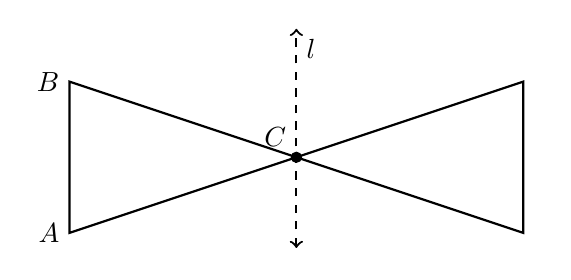
\begin{tikzpicture}[scale=.48]
      %\draw [help lines] (-8,-8) grid (7,5);
      %\draw [thick, <->] (-8.4,0) -- (7.4,0) node [right] {$x$};
      \draw [thick, <->, dashed] (0,-5.4)--(0,0.4) node [below right] {$l$};  
      \draw [thick]
        (-6,-1) node[left] {$B$}--
        (-6,-5) node[left] {$A$}--
        (0,-3) node[above left] {$C$}--cycle;
      \fill (0,-3) circle[radius=0.15cm];
      \draw [thick]
      (6,-1) node[right] {}--
      (6,-5) node[above right] {}--
      (0,-3) node[below right] {}--cycle;
    \end{tikzpicture} \hspace{1cm}
    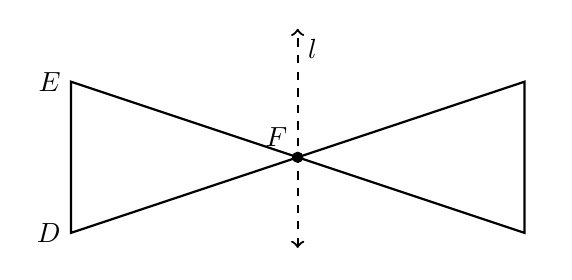
\begin{tikzpicture}[scale=.48]
      %\draw [help lines] (-8,-8) grid (7,5);
      %\draw [thick, <->] (-8.4,0) -- (7.4,0) node [right] {$x$};
      \draw [thick, <->, dashed] (0,-5.4)--(0,0.4) node [below right] {$l$};  
      \draw [thick]
        (-6,-1) node[left] {$E$}--
        (-6,-5) node[left] {$D$}--
        (0,-3) node[above left] {$F$}--cycle;
      \fill (0,-3) circle[radius=0.15cm];
      \draw [thick]
      (6,-1) node[right] {}--
      (6,-5) node[above right] {}--
      (0,-3) node[below right] {}--cycle;
    \end{tikzpicture}
  \end{center} \vspace{1cm}

  \item Find the coordinates of the image of the point $G(6,1)$ after a rotation of $90^\circ$ around the origin.

\end{enumerate}
\end{document}

